\documentclass[border=10pt]{standalone}

\usepackage{tikz}
\usetikzlibrary{arrows,shapes,positioning,shadows,trees}

\renewcommand\familydefault{\sfdefault}

\tikzset{
  basic/.style  = {draw, text width=4cm, drop shadow, font=\sffamily, rectangle},
  root/.style   = {basic, rounded corners=2pt, thin, align=center,
                   fill=gray!20},
  level 2/.style = {basic, rounded corners=6pt, thin,align=center, fill=gray!5,
                   text width=8em},
  level 3/.style = {basic, thin, align=left, fill=gray!0, text width=5em}
}

\begin{document}
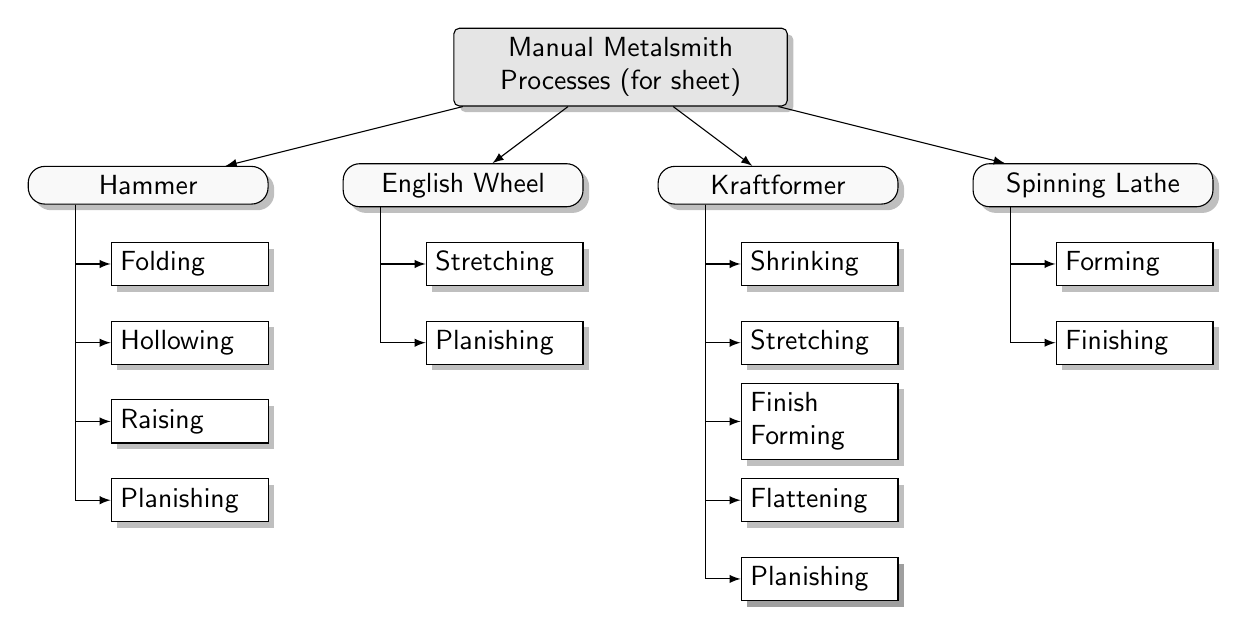
\begin{tikzpicture}[
  level 1/.style={sibling distance=40mm},
  edge from parent/.style={->,draw},
  >=latex]

% root of the the initial tree, level 1
\node[root] {Manual Metalsmith Processes (for sheet)}
% The first level, as children of the initial tree
  child {node[level 2] (c1) {Hammer}}
  child {node[level 2] (c2) {English Wheel}}
  child {node[level 2] (c3) {Kraftformer}}
  child {node[level 2] (c4) {Spinning Lathe}};

% The second level, relatively positioned nodes
\begin{scope}[every node/.style={level 3}]
\node [below of = c1, xshift=15pt] (c11) {Folding};
\node [below of = c11] (c12) {Hollowing};
\node [below of = c12] (c13) {Raising};
\node [below of = c13] (c14) {Planishing};

\node [below of = c2, xshift=15pt] (c21) {Stretching};
\node [below of = c21] (c22) {Planishing};

\node [below of = c3, xshift=15pt] (c31) {Shrinking};
\node [below of = c31] (c32) {Stretching};
\node [below of = c32] (c33) {Finish Forming};
\node [below of = c33] (c34) {Flattening};
\node [below of = c34] (c35) {Doming};
\node [below of = c34] (c36) {Planishing};

\node [below of = c4, xshift=15pt] (c41) {Forming};
\node [below of = c41] (c42) {Finishing};
\end{scope}

% lines from each level 1 node to every one of its "children"
\foreach \value in {1,2,...,4}
  \draw[->] (c1.195) |- (c1\value.west);

\foreach \value in {1,...,2}
  \draw[->] (c2.195) |- (c2\value.west);

\foreach \value in {1,...,5}
  \draw[->] (c3.195) |- (c3\value.west);
  
\foreach \value in {1,2}
  \draw[->] (c4.195) |- (c4\value.west);
\end{tikzpicture}
\end{document}